\documentclass[journal, a4paper]{IEEEtran}
%\IEEEoverridecommandlockouts
% The preceding line is only needed to identify funding in the first footnote. If that is unneeded, please comment it out.

\usepackage{cite}
\usepackage{amsmath,amssymb,amsfonts}
\usepackage{algorithm}
\usepackage{algorithmic}
\usepackage{bm}
\usepackage{graphicx}
\graphicspath{{../figures/}}
\DeclareGraphicsExtensions{.pdf,.jpeg,.png}
\usepackage[caption=false,font=footnotesize]{subfig}
\usepackage{textcomp}
\usepackage[dvipsnames]{xcolor}
\usepackage{systeme}
%\usepackage{IEEEtrantools}

%% Custom Additions
\usepackage{array}
%\usepackage{caption,subcaption}
\usepackage{datetime}
\usepackage{mathtools}
\usepackage{hyperref}
\usepackage{cleveref}
\usepackage{fontawesome5}
\usepackage{lipsum}
\usepackage{mleftright}
\usepackage{optidef}
\usepackage{physics}
\usepackage{xfrac}
%\usepackage[utf8]{inputenc}
%\usepackage[english]{babel}
%\usepackage{float}

% BibTeX
\def\BibTeX{{\rm B\kern-.05em{\sc i\kern-.025em b}\kern-.08em
		T\kern-.1667em\lower.7ex\hbox{E}\kern-.125emX}}

% Theorems
\newtheorem{theorem}{Theorem}[section]

% Floor and ceiling functions
\DeclarePairedDelimiter\ceil{\lceil}{\rceil}
\DeclarePairedDelimiter\floor{\lfloor}{\rfloor}

%% Front matter stuff
\title{A Consumer Appliance-Level Framework\\for Optimized Load Shedding}

%\author{
%	\IEEEauthorblockN{
%		Christian Y. Cahig\IEEEauthorrefmark{1}, Abdul Aziz G. Mabaning\IEEEauthorrefmark{2} \\
%	}
%	\IEEEauthorblockA{
%		\textit{Department of Electrical Engineering and Technology, College of Engineering and Technology}\\
%		\textit{Mindanao State University - Iligan Institute of Technology}\\
%		\IEEEauthorrefmark{1}chriscahig@gmail.com,
%		\IEEEauthorrefmark{2}mraaguevarra@gmail.com
%	}
%}

\author{
	Christian.~Y.~Cahig \textsuperscript{\faIcon[regular]{envelope}}, Abdul~Aziz~G.~Mabaning%
\thanks{
	The authors are with the Department of Electrical Engineering and Technology,
	Mindanao State University - Iligan Institute of Technology,
	Iligan City, Philippines.
}%
\thanks{\faIcon[regular]{envelope} {\color{blue}christian.cahig@g.msuiit.edu.ph}}%
\thanks{\faIcon{github} Project page: {\color{blue}https://github.com/christian-cahig/CALOLS}}
}

%% Document
\begin{document}

\maketitle

\noindent
\textit{Updated as of {\today\ \currenttime}.}\\

\begin{abstract}
% TO DO: Update as often as necessary
Load shedding can be the most viable solution for a utility in scenarios where the balance between power supply and demand is at risk.
As it directly tampers a consumer's access to amenities and benefits, load shedding has to be an optimized process.
This paper retells a recently proposed framework where the smallest sheddable unit of load is a consumer appliance.
The value proposition of such setup is two-fold:
the consumer can avoid total interruption of comfort and productivity,
and the utility can maximize the utilization of available supply.
We also critique the orignally proposed framework
and identify three gaps regarding
the optimization problem formulation,
the solution method, and
the case study scenarios.
We propose methodologies to address the said gaps
and present experiments on synthetic datasets to illustrate our concerns.
Lastly, we make this work entirely available to the public.
\end{abstract}

\begin{IEEEkeywords}
Optimization, power systems, optimal load shedding.
\end{IEEEkeywords}

\section{Introduction}
\label{sec: Introduction}

Load shedding is a course of action a utility company can take
when the balance between power supply and demand is at risk \cite{Jabian2018},
or when the system voltage or frequency exceeds its allowable lower limit for more than a minute \cite{GMC2016}.
Compared to investing on the installation of generating capacities to curb threats on the supply-demand balance,
load shedding is more economical and realistic in short-term considerations.

Since this strategy directly deals with the customers, load shedding has to be an optimized process.
As such, one can find numerous works in literature
(\textit{e.g.},
fast load shedding \cite{Wester2014},
clustering-based load shedding \cite{Potel2019}, and
load shedding during disaster events \cite{Babaei2020})
on feeder-level implementations.
In this setting, the smallest ``sheddable" unit of load is the total load connected to a feeder.
This coarse treatment is prone to excessive shedding of load and an unoptimized utilization of available supply.
Accordingly, we see works on residence-level implementation:
\textit{e.g.},
using smart meters, single-board computers, server monitoring \cite{Bhattacherjee2019},
detecting rate-of-change of frequency \cite{Sigrist2015},
and using a mobile distribution-level PMU \cite{Yao2020}.

Moving forward in this trend, \cite{Jabian2020} proposed a shedding framework where the smallest ``sheddable" unit of load is a consumer appliance.
This granular scheme addresses the concern of excessive load dropping in a feeder-level implementation,
as well as improves the operation of a residence-level setup.
Keeping both the utility and the customer in the framework means both parties can make the most of the situation in their perspectives.
By having the ability to prioritize appliances according to personal judgment, a consumer can avoid total interruption of comfort and/or productivity within his/her premises.
On the other hand, the utility can maximize the utilization of available power supply.

This work is a reimplementation of the framework originally proposed by \cite{Jabian2020}
and is part of the curricular requirements of an academic course on Optimization in Power Systems.
Although we are building on the basic formulation in \cite{Jabian2020},
this present work differs in a number of ways.
First, we critique the original work and emphasize some methodological rooms for improvement.
Second, as the dataset used in the original study is undisclosed,
we develop synthetic datasets based on the well-known open-sourced test cases
(\textit{e.g.}, IEEE 37-Node Test Feeder \cite{Kersting2001}).
Third, we consider different solution strategies,
in addition to the heuristics-based approach in \cite{Jabian2020},
for the core optimization problem.
% TO DO: Update list of contributions.
Lastly, to promote reproducibility, we make our data files, source codes, and documentation available to the public.

The remainder of this paper proceeds as follows.
Section \ref{sec: Basic Problem Formulation} presents the consumer appliance-level framework
and formulates the core optimization problem.
In Section \ref{sec: A Critique of the Original Work}, we discuss a critique of the original work of \cite{Jabian2020}
and propose some methods to address the identified issues.
Section \ref{sec: Datasets} details the procedures for developing the datasets
as well as benchmarks for different scenarios.
% TO DO: Update overview of sections.
Section \ref{sec: Conclusion} concludes the work.

\section{Basic Problem Formulation}
\label{sec: Basic Problem Formulation}

% Section introduction
This section expounds the load shedding framework whose core notion is that a consumer appliance is the smallest ``sheddable'' unit of load.
We first present in Section \ref{subsec: I. System Configuration} how the distribution system is
modelled in terms of how the utility and the consumers participate in the framework.
We then describe in Section \ref{subsec: I. Nomination of Appliances for Load Shedding} the process of nominating appliances as loads to be shed,
which involves two optimization tasks: one on the consumer's side and one on the utility's.
The consumer-side problem is formulated in Section \ref{subsec: I. Consumer-side Optimization}
and the utility-side in Section \ref{subsec: I. Utility-side Optimization}.
More importanty, we remind the reader that this framework is orginally proposed by \cite{Jabian2020},
and that this section is merely a retelling of their novelty.

\subsection{System Configuration}
\label{subsec: I. System Configuration}

Consider a distribution system with $C$ loads (see Fig. \ref{fig: System configuration}),
where each load $c$ represents a consumer (\textit{i.e.}, a registered customer of the utility).
We assume a communication network that is not wholly centralized:
(i) appliances within the premises of consumer $c$ are monitored and controlled by consumer node $\mathsf{K}_{c}$;
(ii) all consumer nodes communicate with central node $\mathsf{U}$ in the utility side (\textit{e.g.}, housed in a substation); and
(iii) communication between $\mathsf{K}_{c}$'s and $\mathsf{U}$ have a bidirectional protocol.

\begin{figure}[t!]
	\centering
	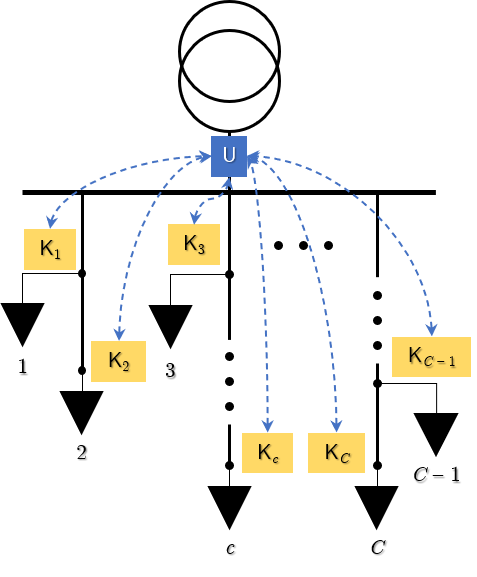
\includegraphics[scale=0.75]{system config.png}
	\caption{System single line diagram and network topology for the consumer appliance-level load shedding.
	Although the figure depicts one load at each node for brevity, the framework presented is not limited to three-phase loads.}
	\label{fig: System configuration}
\end{figure}

For the appliance-level shedding to be possible, a consumer $c$ assigns $P_{c}$ priority levels, according to his/her preference and prerogative (see Fig. \ref{fig: Appliance priority levels}).
In this case, we take $p=1$ as the highest priority of being supplied---\textit{i.e.},
appliances within this priority level are to be supplied first when possible---and
$p=P_{c}$ as the least priority.
There are $M_{p}$ appliances within level $p$, and each of them are denoted by $d_{c,i}^{\left(p\right)}$.
Without introducing another variable, let us use $d_{c,i}^{\left(p\right)}$ as the power rating of that appliance.
We can then represent the appliances in level $p$ by a vector of its power ratings $\mathbf{d}_{c}^{\left(p\right)}$
and the appliances within consumer $c$ as a vector $\mathbf{d}_{c}$,
that is,
\begin{IEEEeqnarray}{rCl}
	\label{eqn: Appliances in a priority level}
	\mathbf{d}_{c}^{\left(p\right)} &=&
	\left[ d_{c,1}^{\left(p\right)}, d_{c,2}^{\left(p\right)}, \ldots, d_{c,M_{p}}^{\left(p\right)} \right]^{\intercal}
	\in \mathbb{R}^{M_{p}} \\
	\label{eqn: Appliances in a consumer}
	\mathbf{d}_{c} &=& 
	\left[ \mathbf{d}_{c}^{\left(1\right)}, \mathbf{d}_{c}^{\left(2\right)}, \ldots, \mathbf{d}_{c}^{\left(P_{c}\right)} \right]^{\intercal}
	\in \mathbb{R}^{N_{c}}
\end{IEEEeqnarray}
where $N_{c} = \sum_{i=1}^{P_{c}} M_{i}$ is the total number of appliances in $c$.
From \eqref{eqn: Appliances in a priority level}-\eqref{eqn: Appliances in a consumer},
it follows that the active power ratings of the appliances add up to
\begin{equation}
	\label{eqn: Sum of appliance ratings for a consumer}
	\sum_{p=1}^{P_{c}} \sum_{i=1}^{M_{p}} d_{c,i}^{\left(p\right)}
\end{equation}

\begin{figure}[t!]
	\centering
	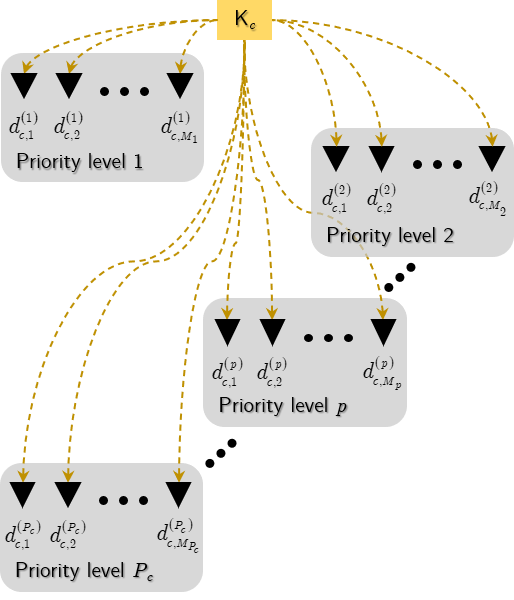
\includegraphics[scale=0.75]{consumer appliance prioritization.png}
	\caption{Grouping of appliances into priority levels for consumer $c$.}
	\label{fig: Appliance priority levels}
\end{figure}

\subsection{Nomination of Appliances for Load Shedding}
\label{subsec: I. Nomination of Appliances for Load Shedding}

In the event where load shedding has to be implemented, the utility has to determine how much load needs to be shed.
If the expected available supply for the system during the impending shedding period is $S_{\text{sys}}$,
and the expected total load during the same period is $L_{\text{sys}}$,
then we can define a \textit{reduction ratio} $\rho$ as
\begin{equation}
	\label{eqn: Reduction ratio}
	\rho = \frac{S_{\text{sys}}}{L_{\text{sys}}}
\end{equation}
Assuming a load shedding scenario where $S_{\text{sys}}$ may not meet $L_{\text{sys}}$,
$\rho$ is the fraction of $L_{\text{sys}}$ that must be shed.
This means that a consumer has to adjust his/her consumption by $\rho - \mu$,
where $\mu$ is a correcting margin\footnote{
$\mu$ can be set as the maximum forecasting error that is likely to happen,
\textit{e.g.}, 95\% of errors in the system's forecast records do not exceed this value.}
determined by the utility to compensate for load forecast errors.
Both $\rho$ and $\mu$ are then communicated by $\mathsf{U}$ to all $\mathsf{K}_{c}$'s.

For a consumer $c$, whose total consumption at the moment $\mathsf{K}_{c}$ receives $\rho$ and $\mu$, is $L_{c}$,
his/her expected supply for the shedding period, $S_{c}$, is given by
\begin{equation}
	\label{eqn: Consumer expected supply}
	S_{c} = \left( \rho - \mu \right) L_{c}
\end{equation}
$\mathsf{K}_{c}$ has to maximize the utilization of $S_{c}$ among all appliances it oversees
according to the priority levels (see Fig. \ref{fig: Utilization of consumer expected supply among appliances}).
At $p=1$, the supply $S_{c}^{\left(1\right)} = S_{c}$ is optimally distributed among appliances $\mathbf{d}_{c}^{\left(1\right)}$.
This results in two groups of appliances for $p=1$:
those that are to be supplied ($\mathbf{p}_{c}^{\left(1\right)}$),
and those that are nominated for shedding ($\mathbf{n}_{c}^{\left(1\right)}$).
Because appliance ratings are fixed and considered indivisible, we can retrieve $\tilde{S}_{c}^{\left(1\right)}$,
which is the portion of $S_{c}^{\left(1\right)}$ that is not allocated to power any more appliances at $p=1$.
Then, $\tilde{S}_{c}^{\left(1\right)}$ becomes the supply to be optimally distributed among appliances at $p=2$
(\textit{i.e.},
$S_{c}^{\left(2\right)} = \tilde{S}_{c}^{\left(1\right)}$)
and the process continues through $p=P_{c}$.
The unallocated supply at the lowest priority level is also the unallocated portion of $S_{c}$,
\textit{i.e.}, $\tilde{S}_{c} = \tilde{S}_{c}^{\left(P_{c}\right)}$.
We can define a vector for all appliances in $c$ ``preliminarily'' nominated for shedding:
\begin{equation}
	\label{eqn: Appliances preliminarily nominated for shedding by a consumer}
	\mathbf{n}_{c} = \left[ \mathbf{n}_{c}^{\left(1\right)}, \mathbf{n}_{c}^{\left(2\right)}, \ldots, \mathbf{n}_{c}^{\left(P_{c}\right)} \right]^{\intercal}
\end{equation}
Then, $\mathsf{K}_{c}$ reports $\tilde{S}_{c}$ and $\mathbf{n}_{c}$ to $\mathsf{U}$.

\begin{figure}[t!]
	\centering
	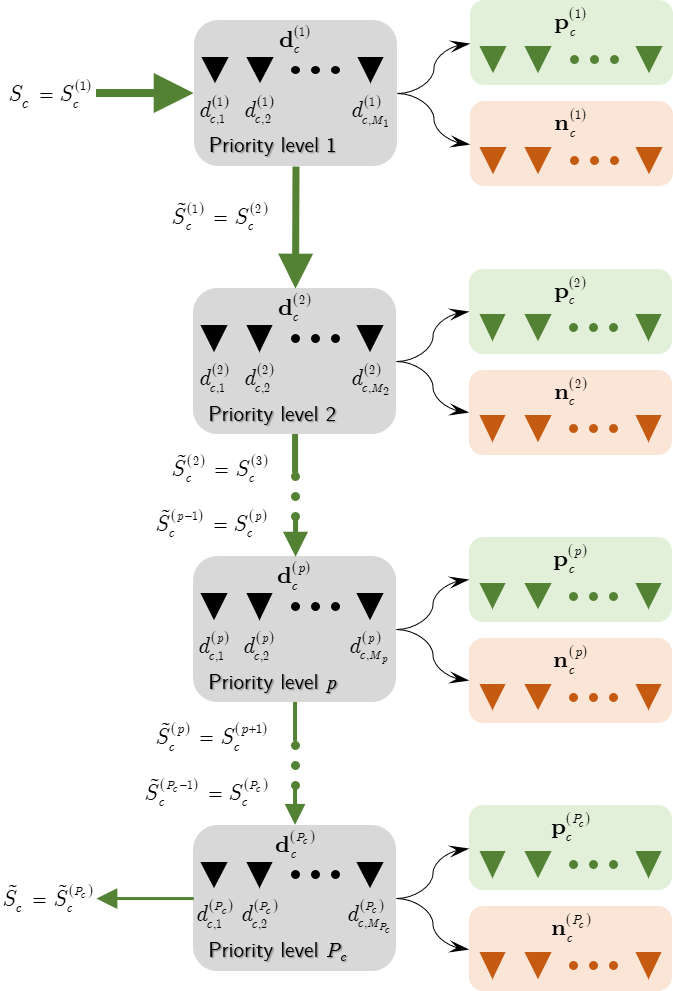
\includegraphics[scale=0.75]{consumer-side optimization.png}
	\caption{Utilization of $S_{c}$ among the appliances of consumer $c$.}
	\label{fig: Utilization of consumer expected supply among appliances}
\end{figure}

Having $\tilde{S}_{c}$ and $\mathbf{n}_{c}$, $\forall c=1,2,\ldots,C$,
we define the total unallocated supply from preliminary nominations $S_{\mathsf{U}}$ and 
the vector of appliances preliminarily nominated for shedding from all consumers $\mathbf{d}_{\mathsf{U}}$ as
\begin{IEEEeqnarray}{rCl}
	\label{eqn: Total unallocated supply from preliminary nominations}
	S_{\mathsf{U}} &=& \sum_{c=1}^{C} \tilde{S}_{c} \\
	\label{eqn: Appliances preliminarily nominated for shedding by all consumers}
	\mathbf{d}_{\mathsf{U}} &=& \left[ \mathbf{n}_{1}, \mathbf{n}_{2}, \ldots, \mathbf{n}_{C} \right]^{\intercal}
\end{IEEEeqnarray}
To further maximize utilization, $\mathsf{U}$ redistributes $S_{\mathsf{U}}$ among $\mathbf{d}_{\mathsf{U}}$
(see Fig. \ref{fig: Utilization of total unallocated supply from preliminarily nominations among preliminarily nominated appliances}).
As with the procedure for each consumer priority level, this results in two groups of appliances:
$\mathbf{p}_{\mathsf{U}}$ contains those in $\mathbf{d}_{\mathsf{U}}$ that are to be supplied using $S_{\mathsf{U}}$,
while $\mathbf{n}_{\mathsf{U}}$ is the final roster of appliances nominated for shedding.
The utility relays $\mathbf{p}_{\mathsf{U}}$ (and/or $\mathbf{n}_{\mathsf{U}}$) to all $\mathsf{K}_{c}$'s.
Then the actual shedding implementation commences.

\begin{figure}[t!]
	\centering
	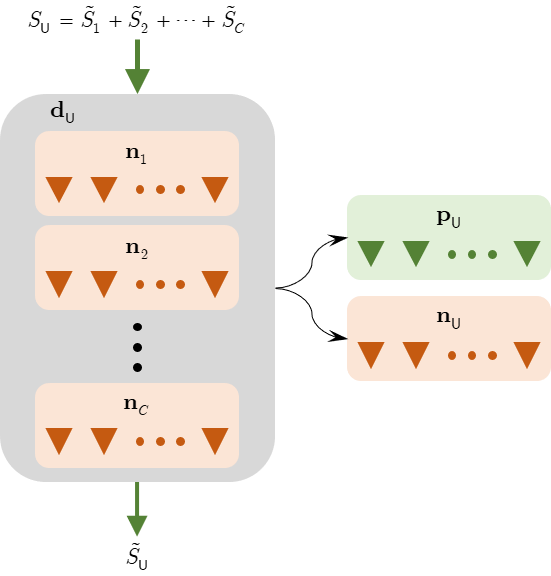
\includegraphics[scale=0.75]{utility-side optimization.png}
	\caption{Utilization of $S_{\mathsf{U}}$ among appliances preliminarily nominated by $\mathsf{K}_{c}$'s.}
	\label{fig: Utilization of total unallocated supply from preliminarily nominations among preliminarily nominated appliances}
\end{figure}

\subsection{Consumer-side Optimization}
\label{subsec: I. Consumer-side Optimization}

At priority level $p$, $\mathsf{K}_{c}$ has to allocate $S_{c}^{\left(p\right)}$ among appliances denoted by $\mathbf{d}_{c}^{\left(p\right)}$.
Each appliance is a quantized load of fixed amount;
hence, $\mathsf{K}_{c}$ can only alter the distribution of $S_{c}^{\left(p\right)}$
by either ``picking up" or nominating for shedding an appliance.
We denote a binary decision variable $k_{i}$
for appliance $d_{c,i}^{\left(p\right)} \in \mathbf{d}_{c}^{\left(p\right)}$
such that
\begin{equation}
	\label{eqn: Consumer-side optimization variable}
	k_{i} =
	\begin{cases*}
		0, & if $d_{c,i}^{\left(p\right)}$ is nominated for shedding \\
		1, & otherwise
	\end{cases*}
\end{equation}

The amount from $S_{c}^{\left(p\right)}$ that is utilized for picking up appliances is given by
\begin{equation}
	\label{eqn: Supply utilized for appliance pick-up in a priority level}
	\begin{split}
		\sum_{i=1}^{M_{p}} k_{i} d_{c,i}^{\left(p\right)} &=\
		k_{1} d_{c,1}^{\left(p\right)} + k_{2} d_{c,2}^{\left(p\right)} + \ldots + k_{M_{p}} d_{c,M_{p}}^{\left(p\right)} \\
		&=\ \left(\mathbf{d}_{c}^{\left(p\right)}\right)^{\intercal} \mathbf{k}
	\end{split}
\end{equation}
where $\mathbf{k} = \left[ k_{1}, k_{2}, \ldots, k_{M_{p}} \right]^{\intercal}$ is the vector representation of the decision variables.
The unallocated portion of $S_{c}^{\left(p\right)}$ is
\begin{IEEEeqnarray}{rCl}
	\label{eqn: Supply not utilized for appliance pick-up in a priority level}
	\tilde{S}_{c}^{\left(p\right)} = S_{c}^{\left(p\right)} - \sum_{i=1}^{M_{p}} k_{i} d_{c,i}^{\left(p\right)} = S_{c}^{\left(p\right)} - \left(\mathbf{d}_{c}^{\left(p\right)}\right)^{\intercal} \mathbf{k}
\end{IEEEeqnarray}
Hence, optimizing the utilization of $S_{c}^{\left(p\right)}$ corresponds to minimizing $\tilde{S}_{c}^{\left(p\right)}$.
In this sense, $S_{c}^{\left(p\right)}$ is a ``cost" to be minimized.
Moreover, one has to restrict the picking up of appliances so that $\tilde{S}_{c}^{\left(p\right)}$ is nonnegative, \textit{i.e.},
\begin{equation}
	\label{eqn: Supply not utilized for appliance pick-up in a priority level must be nonnegative}
	S_{c}^{\left(p\right)} - \left(\mathbf{d}_{c}^{\left(p\right)}\right)^{\intercal} \mathbf{k} \geq 0
\end{equation}

From
\eqref{eqn: Consumer-side optimization variable}-\eqref{eqn: Supply not utilized for appliance pick-up in a priority level must be nonnegative},
the consumer-side optimization problem is
\begin{mini!}|l|
	{ \mathbf{k} }
	{ \left\{ \tilde{S}_{c}^{\left(p\right)} = S_{c}^{\left(p\right)} - \left(\mathbf{d}_{c}^{\left(p\right)}\right)^{\intercal} \mathbf{k} \right\} }
	{\label{eqn: Consumer-side optimization problem}}
	{}{}
	\addConstraint{ S_{c}^{\left(p\right)} - \left(\mathbf{d}_{c}^{\left(p\right)}\right)^{\intercal} \mathbf{k} \geq 0 }
	\addConstraint{ k_{i} \in \left\{0,1\right\},\ i=1,2,\ldots,M_{p} }
\end{mini!}
The solution to \eqref{eqn: Consumer-side optimization problem}, $\mathbf{k}^{\ast}$,
is the switching combinations for appliances $\mathbf{d}_{c}^{\left(p\right)}$
that minimizes $\tilde{S_{c}}^{\left(p\right)}$.
Note that \eqref{eqn: Consumer-side optimization problem} is solved at each priority level $p$ for each consumer $c$.

\subsection{Utility-side Optimization}
\label{subsec: I. Utility-side Optimization}

The distribution of $S_{\mathsf{U}}$ among $\mathbf{d}_{\mathsf{U}}$ is similar to
\eqref{eqn: Consumer-side optimization problem}.
Simply put, utility-side optimization seeks to ``squeeze" out more utilization of supply
with the intuition that $\tilde{S_{c}}$ may be enough to pick up some appliances in $\mathbf{n}_{b}$, $b \neq c$.

Each appliance $d_{\mathsf{U},i} \in \mathbf{d}_{\mathsf{U}}$ can only be controlled by $\mathsf{U}$ in two ways.
We define a binary variable $u_{i}$ to indicate this decision parameter:
\begin{equation}
	\label{eqn: Utility-side optimization variable}
	u_{i} =
	\begin{cases*}
		0, & if $d_{\mathsf{U},i}$ is nominated for shedding \\
		1, & otherwise
	\end{cases*}
\end{equation}
If $\mathbf{d}_{\mathsf{U}}$ has $M_{\mathsf{U}}$ appliances, then the amount from $S_{\mathsf{U}}$ expended for picking up appliances is given by
\begin{equation}
	\label{eqn: Supply utilized for appliance pick-up in utility-side optimization}
	\begin{split}
		\sum_{i=1}^{M_{\mathsf{U}}} u_{i} d_{\mathsf{U},i} &=\
		u_{1} d_{\mathsf{U},1} + u_{2} d_{\mathsf{U},2} + \ldots + u_{M_{\mathsf{U}}} d_{\mathsf{U},M_{\mathsf{U}}} \\
		&=\ \left( \mathbf{d}_{\mathsf{U}} \right)^{\intercal} \mathbf{u}
	\end{split}
\end{equation}
where $\mathbf{u}$ is the vector representation of the decision variables,
and $\mathbf{u}, \mathbf{d}_{\mathsf{U}} \in \mathbb{R}^{M_{\mathsf{U}}}$.
The unallocated portion of $S_{\mathsf{U}}$ is
\begin{equation}
	\label{eqn: Supply not utilized for appliance pick-up in utility-side optimization}
	\tilde{S}_{\mathsf{U}} = S_{\mathsf{U}} - \sum_{i=1}^{M_{\mathsf{U}}} u_{i} d_{\mathsf{U},i} = S_{\mathsf{U}} - \left( \mathbf{d}_{\mathsf{U}} \right)^{\intercal} \mathbf{u}
\end{equation}
where $\tilde{S}_{\mathsf{U}}$ is to be minimized but cannot be negative:
\begin{equation}
	\label{eqn: Supply not utilized for appliance pick-up in utility-side optimization must be nonnegative}
	S_{\mathsf{U}} - \left( \mathbf{d}_{\mathsf{U}} \right)^{\intercal} \mathbf{u} \geq 0
\end{equation}
Finally, the utility-side optimization problem is
\begin{mini!}|l|
	{ \mathbf{k} }
	{ \left\{ \tilde{S}_{\mathsf{U}} = S_{\mathsf{U}} - \left( \mathbf{d}_{\mathsf{U}} \right)^{\intercal} \mathbf{u} \right\} }
	{ \label{eqn: Utility-side optimization problem} }
	{}{}
	\addConstraint{ S_{\mathsf{U}} - \left( \mathbf{d}_{\mathsf{U}} \right)^{\intercal} \mathbf{u} \geq 0 }
	\addConstraint{ u_{i} \in \left\{0,1\right\},\ i=1,2,\ldots,M_{\mathsf{U}} }
\end{mini!}
The solution to \eqref{eqn: Utility-side optimization problem}, $\mathbf{u}^{\ast}$,
is the switching combinations for appliances $\mathbf{d}_{\mathsf{U}}$ that minimizes the $\tilde{S}_{\mathsf{U}}$.

\section{A Critique of the Original Work}
\label{sec: A Critique of the Original Work}

% Section introduction
While the intent of the work by \cite{Jabian2020} is commendable in adding a demand-response dimension to load shedding,
there are certain points in their methodology that we find insufficiently justified
(at least as presented in their paper).
These issues as well as prospective procedures to address them are discussed in the succeeding subsections.

\subsection{On the Cascading Structure of Consumer-side Optimization}
\label{subsec: II. On the Cascading Structure of Consumer-side Optimization}

% TO DO: Update the tenses when accomplished.
The prioritized utilization of $S_c$ (see Fig. \ref{fig: Utilization of consumer expected supply among appliances})
can be recast as a non-cascading procedure.
For example, the priority levels of appliances
$\mathbf{d}_{c} = \left[ d_{c,1}, d_{c,2}, \ldots, d_{c,N_{c}} \right]^{\intercal}$
can be encoded as a vector of corresponding priority weights
$\bm{\phi}_{c} = \left[ \phi_{c,1}, \phi_{c,2}, \ldots, \phi_{c,N_{c}} \right]^{\intercal}$.
In this manner, two appliances $d_{c,i}$ and $d_{c,j}$ are
of the same priority levels if $\phi_{c,i} = \phi_{c,j}$.
Moreover, the consumer-side optimization \eqref{eqn: Consumer-side optimization problem}
need not be performed $P_{c}$ times,
and can be recast as a single-stage minimization of $\tilde{S_{c}}$:
\begin{maxi!}|l|
	{ \mathbf{k} }
	{ \left\{ \tilde{S}_{c} = S_{c} - \left( \bm{\phi_{c}} \odot \mathbf{d}_{c} \right)^{\intercal} \mathbf{k} \right\} }
	{ \label{eqn: Single-stage consumer-side optimization problem} }
	{}{}
	\addConstraint{ S_{c} - \left( \bm{\phi_{c}} \odot \mathbf{d}_{c} \right)^{\intercal} \mathbf{k} \geq 0 }
	\addConstraint{ k_{i} \in \left\{0,1\right\},\ i=1,2,\ldots,N_{c} }
\end{maxi!}
where $\odot$ denotes element-wise multiplication,
and $\mathbf{k} = \left[k_{1}, k_{2}, \ldots, k_{N_{c}} \right]$ is a modified vector representation of the decision variables corresponding to $\mathbf{d}_{c}$.

% TO DO: Update the tenses when accomplished.
Although there is a burden in properly setting $\bm{\phi_{c}}$,
it is reasonable to wonder whether the computational burden of per-priority level optimization
\eqref{eqn: Consumer-side optimization problem}
is significantly less than that of \eqref{eqn: Single-stage consumer-side optimization problem} or any variants thereof.
A possible approach for setting $\bm{\phi_{c}}$ is as follows:
\begin{enumerate}
	\item Create a histogram of the appliance ratings $\mathbf{d}_{c}$ where the number of bins is equal to $P_c$.
	\item Suppose that the sums of the appliance ratings within the bins are $b_{c,P_{c}}, \ldots, b_{c,2}, b_{c,1}$,
	where $b_{c,1} > b_{c,2} > \ldots > b_{c,P_{c}}$.
	\item The priority weight $\phi_{c,i}$ for appliance $d_{c,i}$ with priority level $p$ would be
	\begin{equation*}
		\phi_{c,i} = \frac{b_{c,p}}{\sum_{j=1}^{N_c} d_{c,j}}
	\end{equation*}
\end{enumerate}
This basically weights the appliance rating $d_{c,i}$ with a unitless factor $\phi_{c,i}$
so that the values of the objective and constraint functions
in \eqref{eqn: Consumer-side optimization problem}
and in \eqref{eqn: Single-stage consumer-side optimization problem}
have the same physical units.

\subsection{On the Rush to Heuristics}
\label{subsec: II. On the Rush to Heuristics}

The ``rush to heuristics" may have been unjustified at worst and improvable at best.
In \cite{Jabian2020}, genetic algorithm (GA) and binary particle swarm optimization (BPSO)
with modified initialization schemes were used as the solution method.
The consumer-side \eqref{eqn: Consumer-side optimization problem}
and utility-side \eqref{eqn: Utility-side optimization problem}
optimization are integer linear programming problems,
which can be solved efficiently by properly chosen numerical approaches.
This makes the authors' claim of GA being more suitable than BPSO for real-time applications
of less confidence.
% TO DO: Update the tenses when accomplished.
To address this methodological gap, we consider a comparison of GA and BPSO
with performant numerical approaches such as linear programming relaxation with Gomory cuts
and $\ell_{1}$ regularization.

% TO DO: Update the tenses when accomplished.
We also emphasize that the procedure for tuning GA and BPSO parameters
(\textit{e.g.}, population size, mutation rate, crossover rate, inertia weight)
was not discussed in the original paper.
These parameters are known to affect search performance and quality of results.
We propose an ablation study of these parameters in order to highlight their effects in solving the optimization tasks.

\subsection{On Case Study Scenarios}
\label{subsec: II. On Case Study Scenarios}

Given the implications of future real-life implementation,
the case studies should have included more scenarios
in addition to having ``low" and ``high" diversity of appliance ratings.
Equally pressing scenarios could be varying number of consumer appliances and fixed/varied number of priority levels.
A more serious lapse is that the case studies did not indicate the ground truth optimum values.
This raises a valid concern mainly because GA and BPSO
(among other evolutionary and population-based heuristics)
are known to provide sub-optimal and/or inconsistent results due to reliance on some form of random distribution.

% TO DO: Update the tenses when accomplished.
We address this concern by developing datasets from one common test case but with varying $N_c$ and $P_c$.
Since the data from the actual distribution utility used in \cite{Jabian2020} are undisclosed,
we resort to well-known open-sourced power system test cases.
% TO DO: Update the tenses when accomplished.
We also propose to conduct benchmarks on these datasets considering different metrics
(\textit{e.g.}, optimal $\tilde{S}_{c}^{\left(p\right)}$ for all $p$ and $c$ \eqref{eqn: Consumer-side optimization problem}
and/or $\tilde{S}_{\mathsf{U}}$ \eqref{eqn: Utility-side optimization problem}
considering various $\rho$ and $\mu$ \eqref{eqn: Reduction ratio}-\eqref{eqn: Consumer expected supply}).

\section{Datasets}
\label{sec: Datasets}

% TO DO: Section introduction
Our datasets are based on the IEEE 37-Node Test Feeder\footnote{
	Data files are obtained from IEEE PES's list of test feeders:
	\url{https://site.ieee.org/pes-testfeeders/resources/}.
}
(37NTF) \cite{Kersting2001}.
In Section \ref{subsec: III. Preparation}, we describe the procedure in modifying 37NTF and deriving the datasets.
% TO DO: Update the tenses when accomplished.
Section \ref{subsec: III. Benchmarks} discusses the benchmark tests performed on the datasets.
% TO DO: Update the tenses when accomplished.
Source codes and related files will be available in \texttt{Dataset/} within the project repository.

\subsection{Preparation}
\label{subsec: III. Preparation}

Being a delta-connected system, 37NTF have point loads drawing unbalanced power across phases A-B, B-C, and C-A at their respective nodes.
We treat each phase of a point load in 37NTF as one consumer, provided that it has a non-zero active power value.
For example, the load at node ``742'' which draws active powers of 8 kW across A-B and 85 kW across B-C
is encoded as consumers ``742-1'' and ``742-2'' with respective $L_{c}$'s of 8 kW and 85 kW.
There are 32 consumers in total.
Information about the consumers and their respective power demands are available in the spreadsheet file
\texttt{Dataset/Ported Load Values.xlsx}.

For simplicity, we assume that a consumer $c$'s appliance active power ratings add up to $L_c$, that is,
\begin{equation*}
	L_{c} = \sum_{p=1}^{P_{c}} \sum_{i=1}^{M_{p}} d_{c,i}^{\left(p\right)}
\end{equation*}
To assign power ratings for the $N_{c}$ appliances, we map the interval $\left[0, L_{c}\right]$ unto $\left[0, 1\right]$,
and sample $N_{c} - 1$ points within $\left[0, 1\right]$
according to the continuous uniform distribution $U \left[0.05, 1\right)$,
thereby dividing $\left[0, 1\right]$ (and consequently $\left[0, L_{c}\right]$) into $N_{c}$ sub-intervals.
The length of a sub-interval in $\left[0, 1\right]$ is the active power rating of an appliance
expressed as a fraction of $L_{c}$.
In principle, the lengths of the equivalent sub-intervals in $\left[0, L_{c}\right]$
(that is, the appliance active power ratings) add up to $L_{c}$.
Considering numerical precision, appliance ratings are rounded to 5 decimal places,
and the deficit between $L_{c}$ and the sum of the rounded ratings is added to the rating of a randomly chosen appliance.
Each appliance is then assigned a priority level $p$ drawn from a discrete uniform distribution
$U_{d} \left[1, P_{c}\right]$.

Our treatment of $L_{c}$ and how it is divided into $N_{c}$ appliance ratings is
independent of the unit for active power used by 37NTF (or any originating test case).
Although this does not reflect the active distribution of appliance ratings in practice,
it is sufficient for investigating the concerns raised in Section \ref{subsec: II. On Case Study Scenarios}.
We then prepare three datasets (namely, \textit{37NTF-A}, \textit{37NTF-B}, and \textit{37NTF-C})
that differ in terms of $N_{c}$ and $P_{c}$.
All procedures are accomplished using NumPy \cite{NumPy2020}
and pandas \cite{Pandas2010,Pandas2020},
and are documented in \texttt{Dataset/Preparation.ipynb}.

In 37NTF-A, consumers have the same number of appliances and number of priority levels:
$N_{c} = 100$ and $P_{c} = 5$.
This does not mean consumers have identical appliances or the same number of appliances in a priority level
(see Fig. \ref{fig: Quantitative summaries for 37NTF-A}).
37NTF-A can be accessed via the file \texttt{Dataset/37NTF-A.xlsx}.

In 37NTF-B, all consumers have the same number of priority levels: $P_{c} = 5$.
However, the consumer with the largest active power demand (say, $\hat{L_{c}}$)
has the most number of appliances, $\hat{N_{c}} = 100$.
For all other consumers, the number of appliances is given by
\begin{equation*}
	N_{c} = \floor*{\frac{L_{c}}{\hat{L_{c}}} \hat{N_{c}}} + U_{d} \left[10,20\right]
\end{equation*}
The intuition for this scenario is that the consumer with the largest demand can be expected to have the most number of appliances
(see Fig. \ref{fig: Quantitative summaries for 37NTF-B}).
37NTF-B is stored as a spreadsheet file \texttt{Dataset/37NTF-B.xlsx}.

In 37NTF-C, all consumers have the same number of appliances: $N_{c} = 100$.
They only differ in the number of priority levels;
for a consumer $c$, $P_{c}$ is drawn from $U_{d} \left[1,5\right]$.
This scenario seeks to capture the heterogeneity of consumer preference in terms of appliance prioritization
(see Fig. \ref{fig: Quantitative summaries for 37NTF-C}).
A consumer with $P_{c} = 5$ could be someone who prefers some appliances to be picked up first before others.
On the other end, $P_{c} = 1$ means consumer $c$ treats all appliances equally important to be picked up.
37NTF-C is available as a spreadsheet file \texttt{Dataset/37NTF-C.xlsx}.

\begin{figure*}[t!]
	\centering
	\subfloat[\label{fig: Quantitative summaries for 37NTF-A: TRPL}]{
		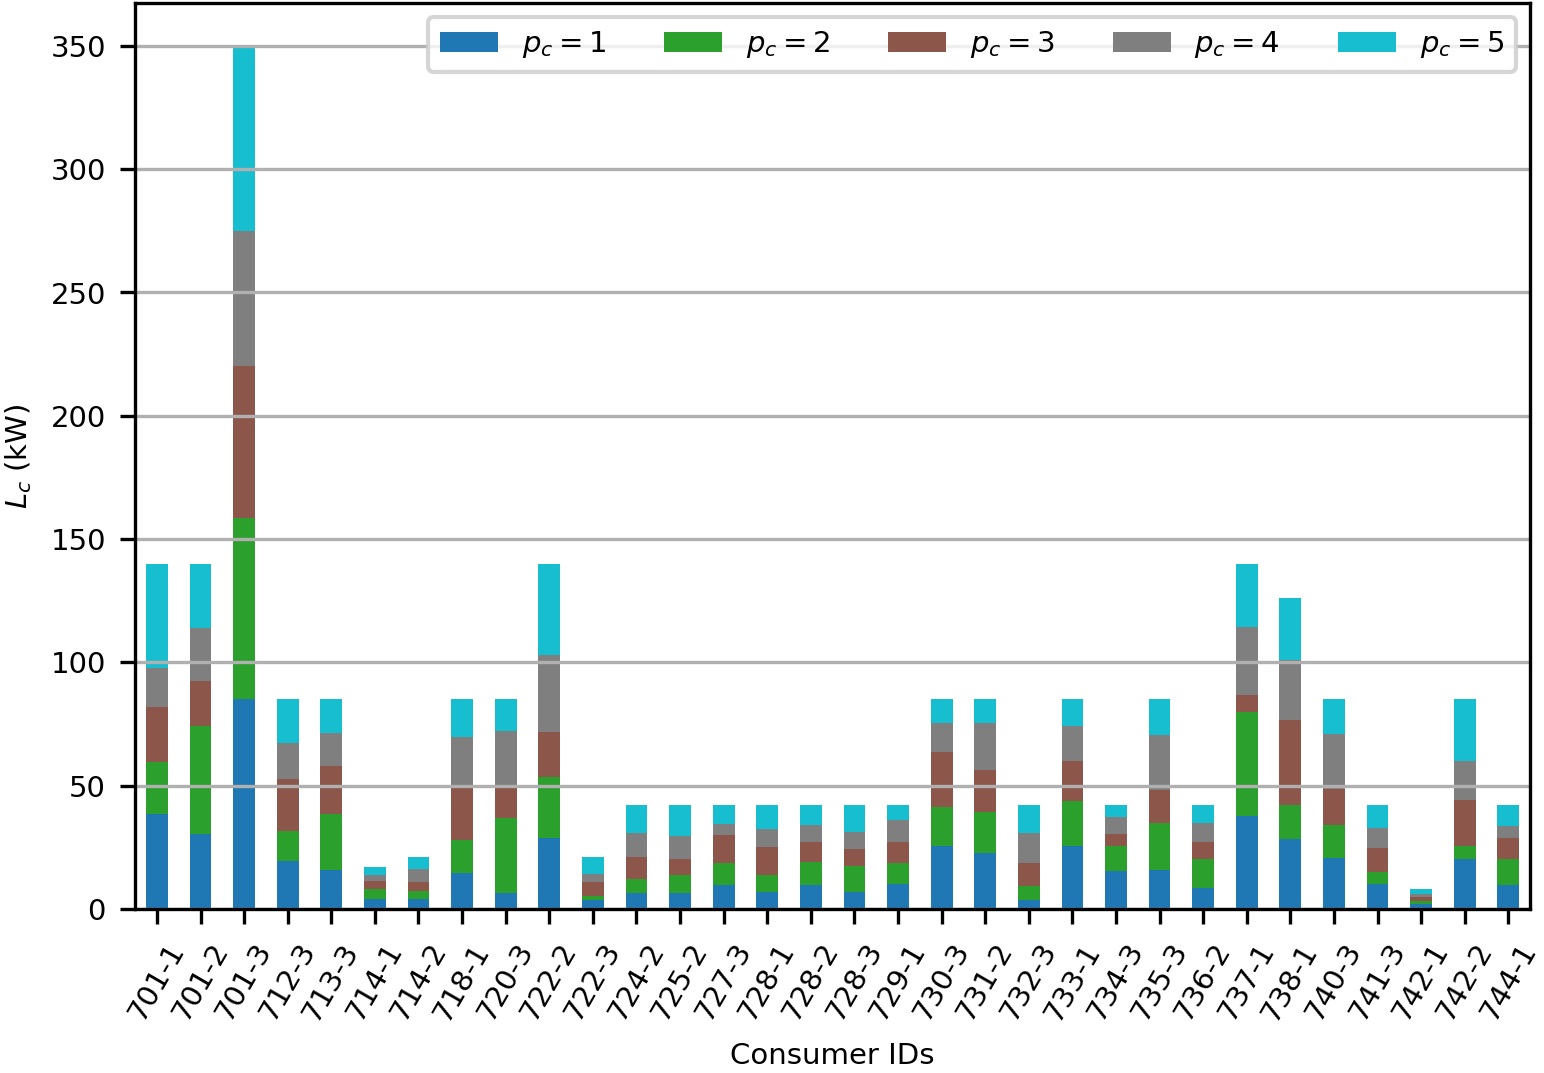
\includegraphics[width=0.49\textwidth]{37NTF-A TRPL}
	}
	\subfloat[\label{fig: Quantitative summaries for 37NTF-A: ACPL}]{
		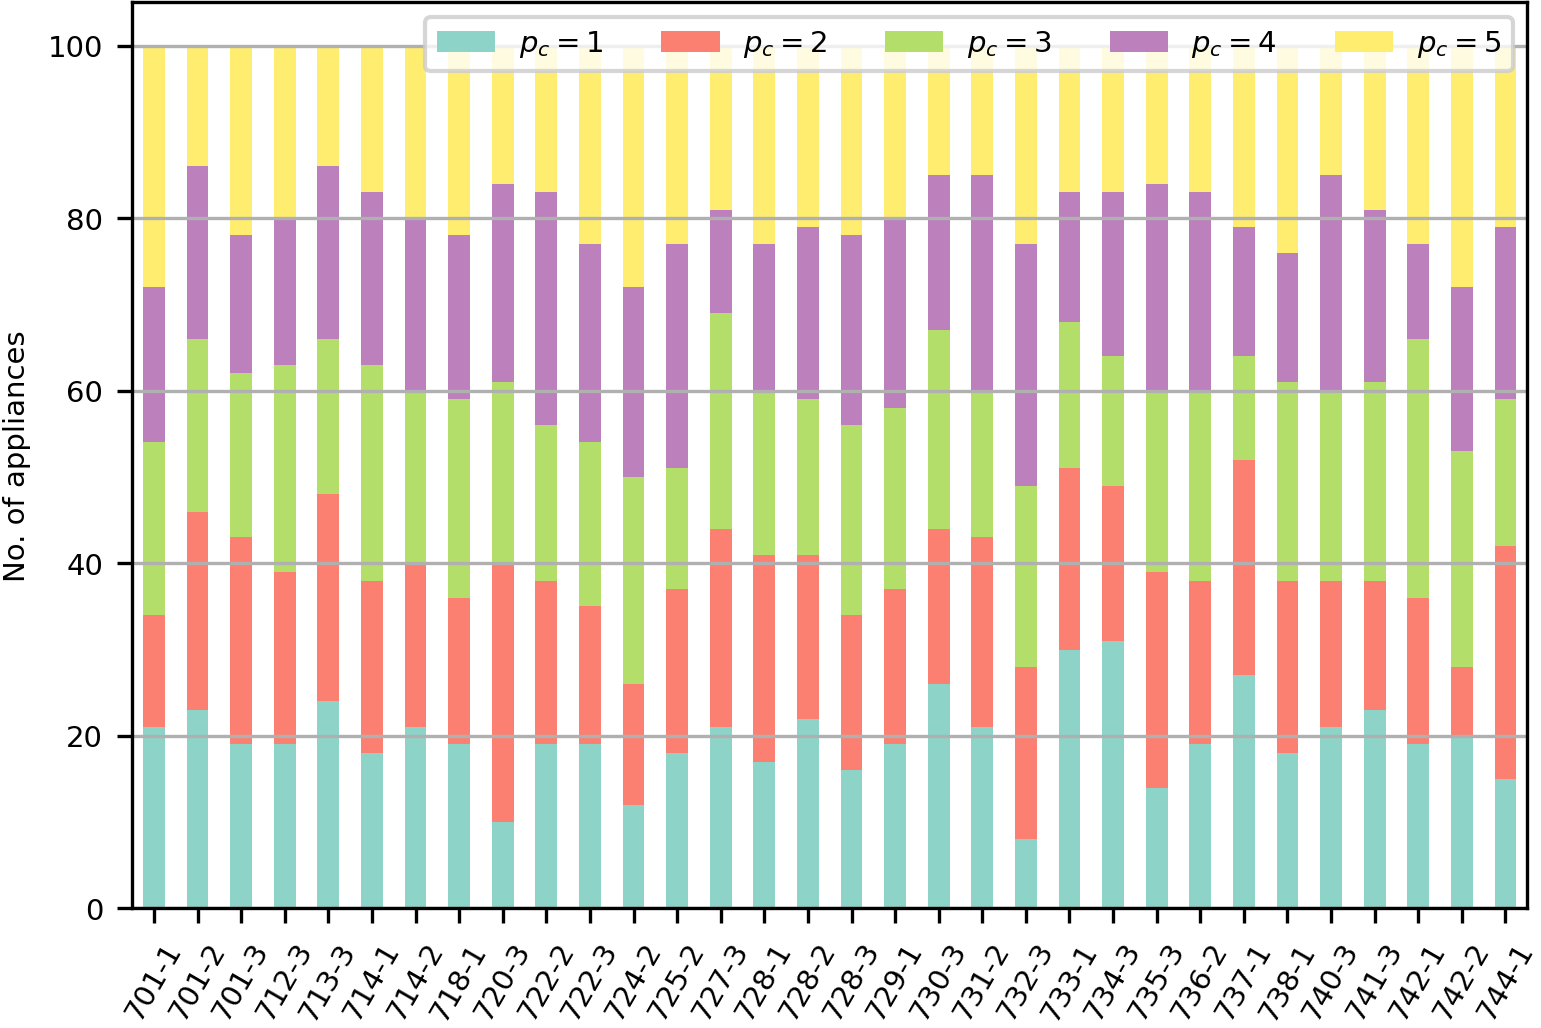
\includegraphics[width=0.49\textwidth]{37NTF-A ACPL}
	}
	\caption{
		Quantitative summaries for 37NTF-A:
		distribution of $L_{c}$ (a) and of $N_{c}$ (b)
		across all $p_{c}$'s in all $c$'s.
		Horizontal axis labels are consumer names.
	}
	\label{fig: Quantitative summaries for 37NTF-A}
\end{figure*}

\begin{figure*}[t!]
	\centering
	\subfloat[\label{fig: Quantitative summaries for 37NTF-B: TRPL}]{
		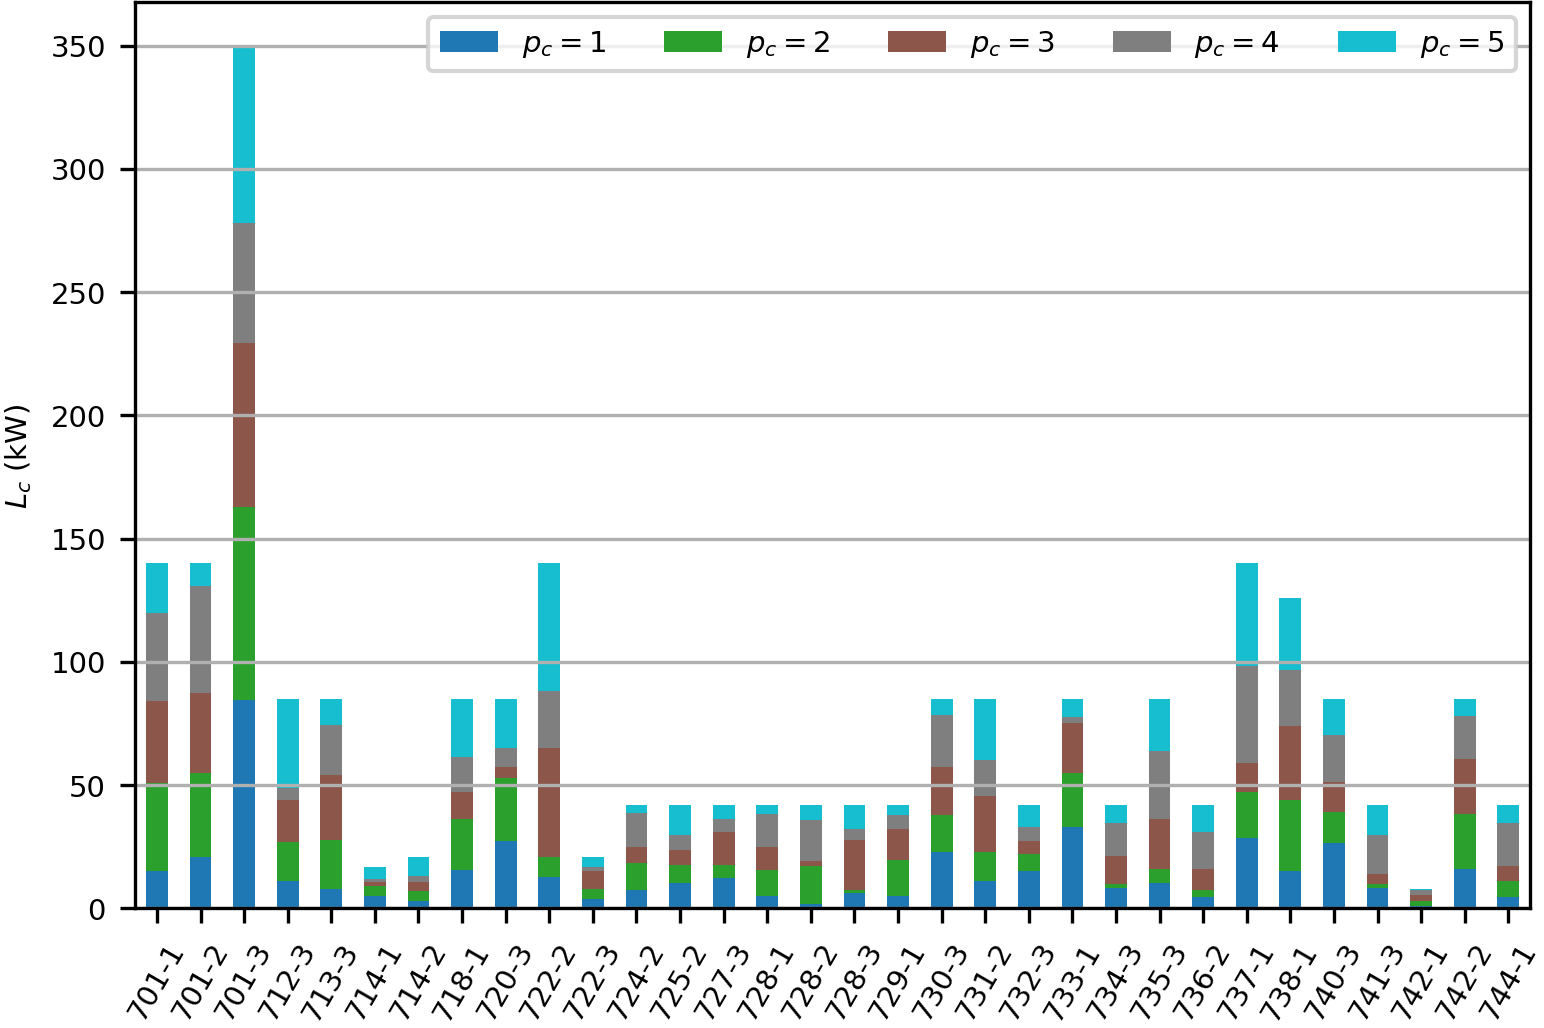
\includegraphics[width=0.49\textwidth]{37NTF-B TRPL}
	}
	\subfloat[\label{fig: Quantitative summaries for 37NTF-B: ACPL}]{
		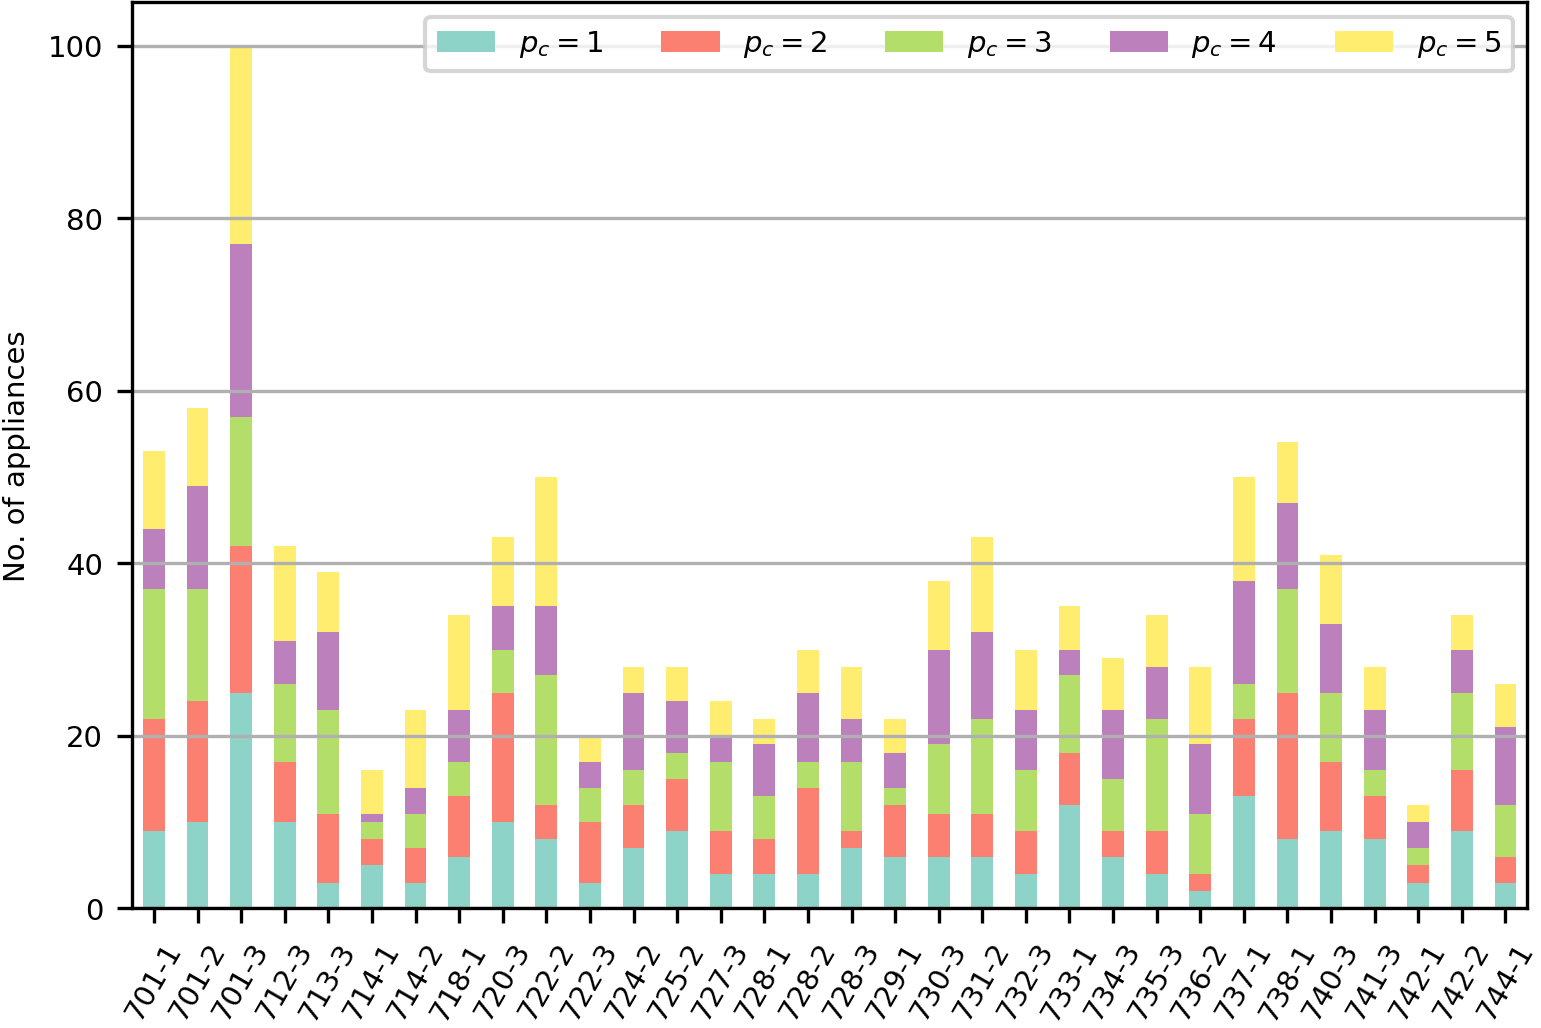
\includegraphics[width=0.49\textwidth]{37NTF-B ACPL}
	}
	\caption{
		Quantitative summaries for 37NTF-B:
		distribution of $L_{c}$ (a) and of $N_{c}$ (b)
		across all $p_{c}$'s in all $c$'s.
		Horizontal axis labels are consumer names.
	}
	\label{fig: Quantitative summaries for 37NTF-B}
\end{figure*}

\begin{figure*}[t!]
	\centering
	\subfloat[\label{fig: Quantitative summaries for 37NTF-C: TRPL}]{
		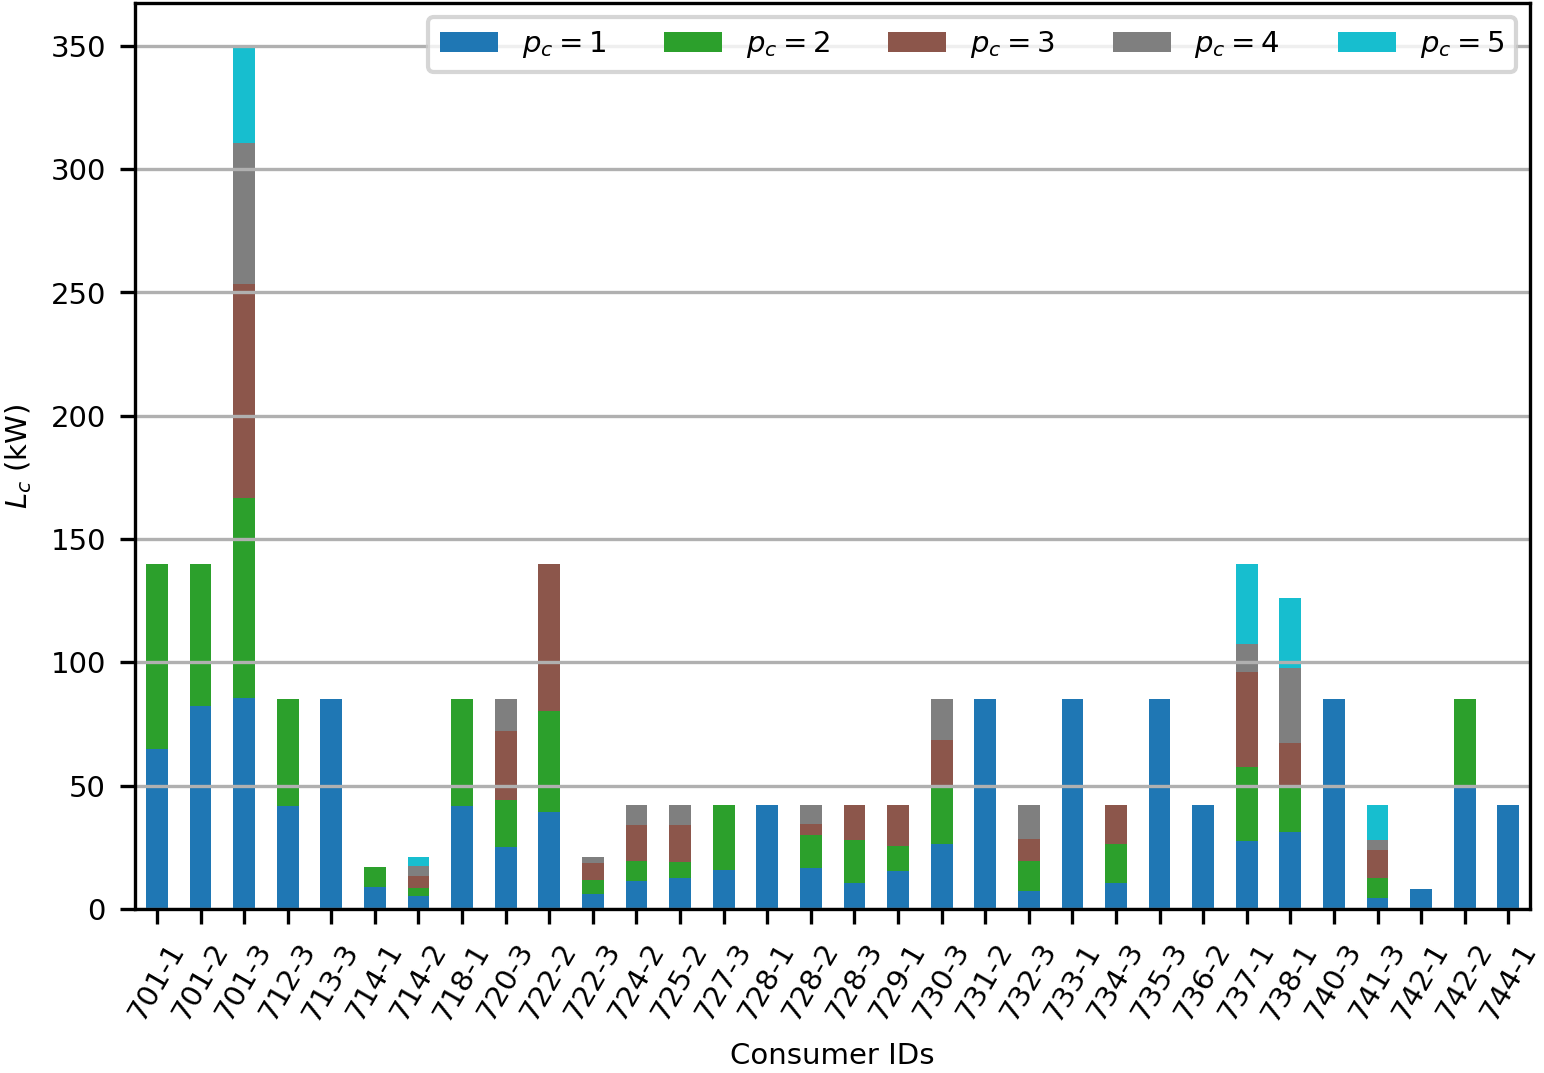
\includegraphics[width=0.49\textwidth]{37NTF-C TRPL}
	}
	\subfloat[\label{fig: Quantitative summaries for 37NTF-C: ACPL}]{
		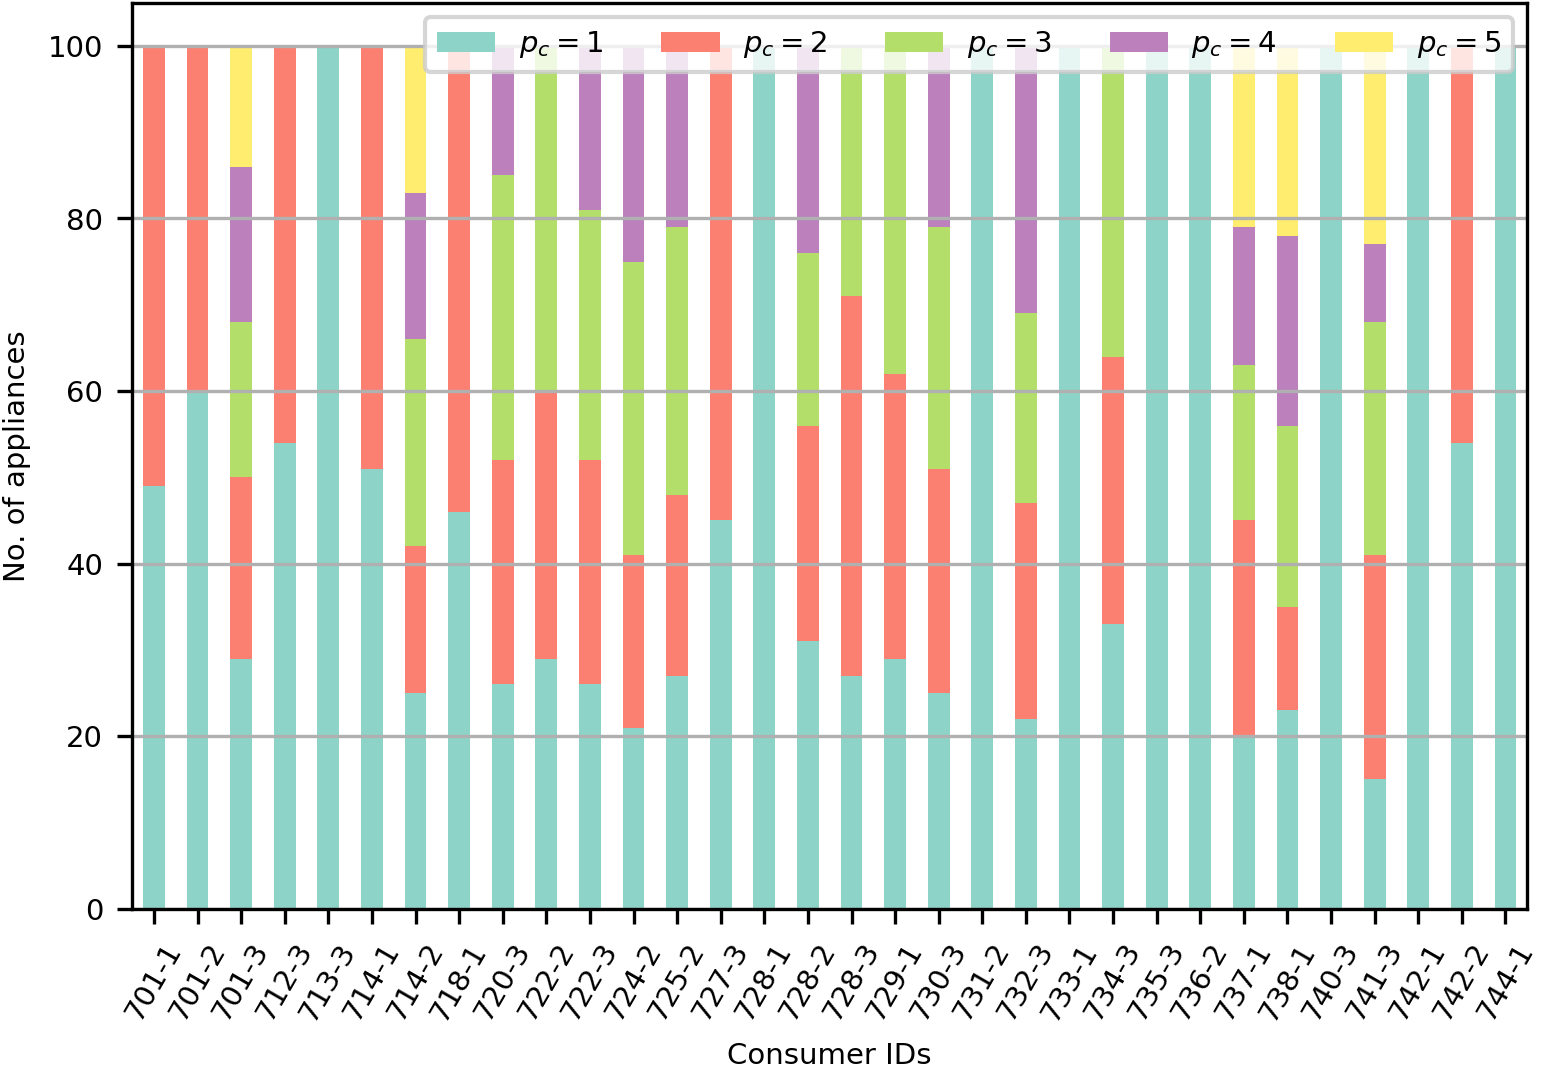
\includegraphics[width=0.49\textwidth]{37NTF-C ACPL}
	}
	\caption{
		Quantitative summaries for 37NTF-C:
		distribution of $L_{c}$ (a) and of $N_{c}$ (b)
		across all $p_{c}$'s in all $c$'s.
		Horizontal axis labels are consumer names.
	}
	\label{fig: Quantitative summaries for 37NTF-C}
\end{figure*}

\subsection{Benchmarks}
\label{subsec: III. Benchmarks}

\lipsum[8]

\section{Conclusion}
\label{sec: Conclusion}

\lipsum[28]

%%%%%%%%%%%%%%%%%%%%%

% Acknolwedgement
%\vspace{40pt}
%\section*{Acknowledgment}

% References
%\vspace{40pt}
%\section*{References}
\bibliographystyle{IEEEtran}
%The argument is your BibTeX string definitions and bibliography database(s).
\bibliography{../references}

\end{document}
